\setchapterstyle{kao}
\setchapterpreamble[u]{\margintoc}

\chapter{Теория NP-полноты}
\labch{mathematics}

\section{Два подхода к сложности задачи}
\labsec{two-difficulty-approarch}
Первый подход предлагает считать сложностью алгоритма число тактов работы
машины, реализующей этот алгоритм (число тактов работы в Машине Тьюринга, число
совершённых подстановок в НАМ, число команд выполненных РАМ).

Второй подход предлагает рассматривать в качестве алгоритма булеву функцию,
реализующую этот алгоритм, и в качестве сложности рассматривать число
функциональных элементов в схеме из функциональных элементов, реализующих эту
функцию. \sidenote{Этот подход рассматривает \refch{functional}.} 

В любом случае понятно, что для разных индивидуальных задач I сложность будет разной. 

Возьмём все индивидуальные задачи $I$ с входом длины $|I| \le m$. Число таких
задач обозначим $Z_n$. Очевидно, что для конечного алфавита число $Z_n$ --- конечно. 

\begin{definition}
	Сложность в худшем назовём $t_Z(n) = \max_{|I|\le n} t(I)$.
\end{definition}
\marginnote[0pt]{Максимальное
	время работы алгоритма на индивидуальных задачах $I$ с длиной входа $|I|
	\le n$.}

\begin{definition}
	Сложностью в среднем назовём \[
		\frac{\sum\limits_{|I|\le n} t\left( I \right) }{Z_n}
	.\] 
\end{definition}

Для каждой задачи может быть сколь угодно много различных алгоритмов $A_Z^1,
A_Z^2, \ldots$. 
\begin{definition}
	Сложность задачи --- наилучшая из сложностей алгоритмов, решающих эту
	задачу.
\end{definition}

\begin{definition}
	Будем называть задачу трудно разрешимой, если у всех алгоритмов,
	решающих её, сложность по меньшей мере экспоненциальная. \cite{Aho}
\end{definition}
Для сравнения масштабов, если 1 такт занимает $10^{-6}$ секунд, то для входа
длины 60 алгоритм со сложностью  $n^6$ будет работать 13 минут, а со сложностью
$2^n$ --- 366 веков.
% \marginnote[-0.7cm]{}

\begin{marginfigure}[-6.5cm]
	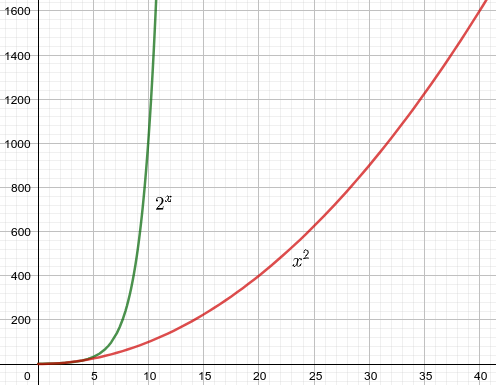
\includegraphics{xpow2and2powx.png}
	\caption{График функций $2^x$ и $x^2$.
	Сравнение графиков функций $x^2$ и  $2^x$ как пример,
насколько сильна разница между экспоненциальной и полиномиальной
сложностью. Сравните рост значений в
окрестности 10, например.
}
\end{marginfigure}

При этом развитие техники на время работы экспоненциальных алгоритмов никак
влиять не будет. Даже при увеличении мощностей в 1000 раз, экспоненциальный
алгоритм будет работать за адекватное время на задаче с длиной входа на 10
символов больше, чем сейчас.\sidenote{Пусть сейчас наибольшая задача, которая решается за
	допустимое время имеет размер n, тогда при увеличении мощностей в 1000
	раз мы имеем прирост в $\log_2 1000 \simeq 10$
}


\section{Определение классов P, NP}
\labsec{P-NP-def}

\begin{definition}
	Слово из входных символов допускается (воспринимается) тогда и только
	тогда, когда машина Тьюринга, начав работу в выделенном начальном
	состоянии, сделаем последовательность шагов, которые в конце концов
	приведут её в допускающее состояние.
\end{definition}
\begin{definition}
	Языком L(M), допускаемым машиной M, называют множество всех цепочек
	(слов) из входных символов, допускаемых M.
\end{definition}

\begin{definition}
	Класс P --- это класс языков, допускаемых МТ за полиномиальное
	время. 
\end{definition}
\marginnote[*-2]{То есть МТ допускает язык и её время работы ограничено
	полиномом.}
Задачи (языки) из класса P называются полиномиально разрешимыми.
\begin{definition}
	Класс NP --- класс языков, допускаемых НМТ за полиномиальное время.
\end{definition}

\begin{theorem}
	Если $Z\in NP$, то существует такой полином  $p(n)$, что Z может быть
	решена на детерминированной МТ за время  $O(2^{p(n)})$.
\end{theorem}
\begin{proof}
Если Z решается на НМТ за полином $q\left( n \right) $, то значит для каждой I
найдётся отгадка U(I) после записи которой НМТ будет работать как обычная МТ и
будет проверять отгадку. Время проверки отгадки, написанной
угадывающей головкой --- $O(q(n))$, а значит и длина отгадки --- $O(q(n))$. 

Для перебора всех отгадок понадобится в алфавите длины k потребуется $k^{q(n)}$,
а значит в сочетании с
проверкой всё займёт $O(k^{q(n)}*q(n)) = O(2^{p(n)})$\sidenote[*]{Просто возьмём
достаточно большой полином}.
\end{proof}

\section{Полиномиальная сводимость}

\begin{definition}
	Язык $L_1 \subset A^*$ сводится к языку $ L_2 \subset B^*$, если
	существует такое отображение $f: A^* \to B^*$, что выполняются два
	условия.
	\begin{enumerate}
		\item Функция f вычисляется за полиномиальное время. (Например,
			существует МТ, которая за полиномиальное число тактов
			вычисляет эту функцию.)
		\item Для любого входа $I\in A^*$ соотношение $I\in L_1$
			выполняется тогда и только тогда, когда выполняется
			соотношение  $f(I)\in~L_2.$
	\end{enumerate}
\end{definition}

\marginnote[-4cm]{
	Мы знаем, что произведение двух полиномов и полином от
	полинома также будет полиноном. Получается, если задача $Z_1$ имеет
	полиномиальную сложность $O(p(n))$, то, если $Z_2$ полиномиально сводится к  $Z_1$
	за $O(q(n))$, то сложность $Z_2$ --- $O(p(q(n))$.\\
	Логично, что если задача может быть
	сведена к другой за время не меньшее, чем экспоненциальное время, то о
	принадлежности одним классам говорить нечего. 
}

Полиномиальную сводимость будем обозначать $\le_P$.


\begin{lemma}
	Если $Z_1 \le_P Z_2$ и  $Z_2 \le_P Z_3$, то $Z_1 \le_P Z_3$
\end{lemma}
\begin{proof}
	Пусть $Z_1 \le_P Z_2$ путём отображения f, а  $Z_2 \le_P Z_3$ --- g.
	Тогда рассмотрим суперпозицию gf, которое будет сводить $Z_1$ к  $Z_3$.
	При этом, так как f и g полиномы, то и их композиция тоже будет
	полиномом.
\end{proof}
\begin{lemma}
\lablemma{polynom-P}
	Пусть $Z_2 \in P$, и  $Z_1 \le_P Z_2$. Тогда  $Z_1 \in P$.
\end{lemma}
\begin{proof}
	Пусть A и B --- алфавиты языков $L_1$ и $L_2$, а функция $f: A^* \to
	B^*$ осуществляет полниномиальную сводимость $L_1$ к $L_2$.

	$Z_2\in P$, значит существует машина Тьюринга $M_2$, решающая  $Z_2$ за
	$O(p(n))$ тактов.
	$M_f$ --- машина Тьюринга, реализующая функцию f, работающая за
	$O(q(n))$ тактов.
	
	Тогда композиция Машин Тьюринга $M_1 = M_2M_t$, которая сначала
	преобразует (сведёт) условие задачи $Z_1$ к условию $Z_2$, а потом решит
	её, будет работать за полином.

\end{proof}
\marginnote[-2.5cm]{Если попросили решить задачу, которая может быть полиномиально сведена к уже
известной задаче из P, то можно радоваться и писать решение за полином.}

\begin{theorem}
Задача нахождения Гамильтонова Цикла\sidenote{Гамильтонов цикл --- цикл в графе,
который проходит по каждой вершине графа ровно один раз} в графе сводится к задаче Комивояжёра.
\end{theorem}
\begin{proof}
На вход в задаче о Гамильтоновом цикле поступает граф G = (V, E). Требуется
ответить на вопрос: существует ли в графе Гамильтонов цикл. 

Входом в задаче Комивояжера является матрица расстояний \[\left( a_{ij}
\right)_{n\times n}
,\] число B. Требуется ответить, существует ли обход\sidenote{посещение каждой
вершины хотя бы по одному разу} по всем вершинам суммарной
длины $\le B$.
\[
n=|V|, B = n, a_{ij} = \begin{cases}
	
	1, \{v_i, v_j\} \in G\\
	2,  \{v_i, v_j\} \notin G
\end{cases}
.\]
Осталось доказать, что гамильтонов цикл в G существует тогда и только тогда,
когда существует обход длины $\le n$. 

$\left( \implies \right) $. Если гамильтонов цикл существует, то всем рёбрам
этого цикла соответствует 1 в $\left( a_{ij} \right) $. А значит обход найдётся. 

$\left( \impliedby \right) $. Очевидно, что, если обход нашёлся, мы прошли по
ребрам длины 1. Значит, в исходном графе мы прошли по существующим рёбрам. Так
как обход подразумевает прохождение по всем вершинам, то мы нашли Гамильтонов
цикл.
\end{proof}
\begin{theorem}
Задача КНФ-выполнимость полиномиально сводится к задаче о клике.
\end{theorem}
\begin{proof}
Прежде всего обозначим вход и вопрос для обеих задач. 

КНФ-выполнимость на вход получает КНФ \[
K(x_1,\ldots,x_n) = \left(x_{i_1}^{\sigma_1} \cup x_{i_2}^{\sigma_2}\cup\ldots\cup
x_{i_p}^{\sigma_p}\right) \&\ldots\left( x_{s_1}^{\kappa_1} \cup
x_{j_2}^{\kappa_2}\cup\ldots\cup x_{j_s}^{\kappa_s} \right)
\] 
Количество скобок в K = m. Вопрос: существует ли такой набор \[
\begin{cases}
	x_1 = v_1\\
	x_2=v_2\\
	\ldots\\
	x_n = v_n\\
\end{cases}
\] такой, что $K(v_1, v_2,\ldots,v_n) = 1$. Другими словами, ответ
"да"{}, если K не тождественный 0.

Задача о клике получает на вход граф $G = (V, E)$, а также число B. Вопрос:
существует ли клика, размера $\ge B$ \sidenote{Клика --- полный подграф.}. 

Пусть V --- множество всех литералов\sidenote{Будем разделять литералы и
	переменные в этом доказательстве. Литералы --- конкретные переменные в
конкретной степени в конкретной скобке КНФ.} в КНФ. При этом даже если $x_1$
содержится в 1й скобке и во 2-й это будут два разных литерала. Примем B = m.
$\{v_i, v_j\} \in G \Leftrightarrow v_i \text{и} v_j$ находятся в разных скобках
и соответствуют либо разным переменным, либо одинаковым переменным в одинаковой
степени.

Докажем, что КНФ выполнима тогда и только тогда, когда построенный нами граф
имеет клику. 

$(\implies)$. Разложим КНФ на дизъюнкцию мономов. Если КНФ выполнима, то хотя бы один из
мономов обращается в 1. Рассмотрим этот моном. Очевидно, что все его литералы
были взяты из разных скобок и, так как он обращается в 1, там нет конъюнкции
двух одинаковых переменных в разных степенях (иначе он был бы тождественным 0).
Получается, что для всех вершин, соответствующих литералам в этом мономе,
проведены рёбра между ними. Значит, этому моному соответствует клика. Размер
монома --- m, значит и размер клики тоже m.

$\left( \impliedby \right) $. Пусть в сгенерированном графе нашлась клика
размерности m. Значит, ей соответствуют m литералов из разных скобок, которые
образуют моном. Так как произведений $x_i \& \overline{x_i}$ быть не может по
условию построения графа, значит этот моном может быть обращён в единицу, а
значит КНФ выполнима.

\end{proof}

\section{Класс NPC}
\labsec{NPC}
\begin{definition}
	Класс NPC (NP Complete) --- класс таких задач, что для любой задачи
	$Z\in NPC$ выполнено условие, что $Z\in NP$ и $\forall Z'\in NP, Z'
	\le_P Z$.
\end{definition}

\begin{lemma}
	Если $Z\in NPC$ и  $Z \le_P Z'$, то  $Z' \in NPC$
\end{lemma}
\marginnote[-0.7cm]{Доказательство этого факта очевидно и прямо следует из
определения.}

\begin{theorem}
\labthm{Cook}
Задача о КНФ-выполнимости --- NPC.
\end{theorem}
\begin{proof}
В данном доказательстве мы не можем пользоваться полиномиальной сводимостью к
другим NPC задачам. Только определением класса NP. Задачу КНФ-выполнимость будем
сокращать в этом доказательстве как КНФ-в.

По сути мы должны доказать, что $\forall Z' \in NP$,  $Z' \le_P$ КНФ-в. 

Задачу $Z'$ можно решить за полином на НМТ, для простоты рассуждений возьмём в
качестве полинома --- $n^k$, где n --- длина входа  $|I|$. \marginnote{Понятно,
что если задача решается за время, меньшее, чем $n^k$, то она может быть
решена и за  $n^k$. }

Зададим часть ограничений на нашу НМТ. Пусть она останавливается только в одном
конечном состоянии $q_{final}$

Рассмотрим ту часть работы НМТ, когда она работает как обычная МТ\sidenote{Далее
под работой МТ будет пониматься именно эта часть}, то есть
отгадка уже написана.\sidenote{Угадывающая головка НМТ работает также за
$O(n^k)$}.

Тогда мы за $n^k$ шагов должны дойти до конечного состояния $q_{filal}$,
проверив отгадку.

Представим работу МТ в виде таблицы, в i-й строке которой записано i-е слово
конфигурации этой МТ.
\begin{table}[htpb]
	\centering
	\label{tab:label}
	\begin{tabular}{|c|c|c|c| c|c|c |c|c|c| c|c|c|c|}
\hline №&$-n^k$& \ldots&\ldots& $-m$& \ldots&$-1$&$0$& $1$ &\ldots&$l$&
		\ldots& \ldots&$n^k$\\
		\hline
		      0&$\lambda$ & \ldots &
		      $\lambda$&$u_m$&\ldots&$u_1$&$q_0$&$v_1$&\ldots&$v_l$
			       &$\lambda$& \ldots&$\lambda$\\\hline
\hline
$n^k$&\ldots&\ldots&\ldots&\ldots&\ldots&\ldots&\ldots&\ldots&$q_{final}$&\ldots&\ldots&\ldots&\ldots\\\hline
	\end{tabular}
\end{table}

Данная таблица конфигурации будет соответствовать МТ при выполнении 4-х условий
одновременно.
\begin{enumerate}
	\item В каждой ячейке содержится один и только один символ из набора $A
		\cup S \cup \{\lambda\}$
	\item В 0-й строке находятся $-n^k - m$ символов  $\lambda$ после идёт m
		символов отгадки $u_m, \ldots, u_1$, начальное состояние $q_0$,  $l$ символов
		условия $v_1, \ldots, v_l$, а после  $n^k-l$ символов  $\lambda$
	\item В $n^k$-й строке есть ячейка, содержащая $q_{final}$
	\item $k$-я и $(k+1)$-я строки различаются не более чем окошком $2\times
		3$, имеющем вид одной из трёх таблиц:
		\marginnote{Окошки соответствуют переходам $qb \to
		q'cR; qb\to q'cSt; qb\to q'cL $}

\begin{table}[h!]
\centering
\begin{tabular}{|c|c|c|}
\hline a&q&b\\
\hline a&c&$q'$\\
\hline
\end{tabular}
\end{table}
\begin{table}[h!]
\centering
\begin{tabular}{|c|c|c|}
\hline a&q&b\\
\hline a&$q'$&c\\
\hline
\end{tabular}
\end{table}
\begin{table}[h!]
\centering
\begin{tabular}{|c|c|c|}
\hline a&q&b\\
\hline $q'$&a&c\\
\hline
\end{tabular}
\end{table}

$a, b, c \in A; q, q' \in S$

\end{enumerate}
Если мы сможем перевести эти четыре утверждения в булеву функцию, то значит мы
свели NP-задачу к КНФ-в., потому что эти 4 условия выполняются тогда и только
тогда, когда МТ успешно проверяет отгадку, а значит ответ на задачу I --- да.

Пусть переменная $x_{i,j,\sigma} =$ 1, если в ячейке  $(i,j)$ таблицы
конфигураций содержится символ  $\sigma$ и = 0 во всех остальных случаях.

Первая формула запишется как \[
	\phi_{line} = \&_{-n^k\le i, j\le n^k} \left( \left( \cup_{\sigma \in A\cup S \cup
	\{\lambda \} } \left( x_{i,j,\sigma}  \right)  \right)\&
	\\
	\left(
	\&_{\substack{\sigma\in A\cup S \cup
	\{\lambda \}
	, \\
\xi\in A\cup S \cup \{\lambda \},\\
\sigma \neq \xi
	}} \left( \overline{x_{i,j,\sigma}} \cdot \overline{x_{i,j,\xi}} \right)
\right) \right)
.\] 

Первая часть отвечает за то, чтобы каждая клетка содержала хотя бы один символ
из допустимого множества, вторая часть, чтобы в каждой клетке находилось не
более одного символа из множества допустимых значений.

Второе утверждение может быть записано формулой:
\[
	\phi_{start} = \left( \&_{\substack{-n^k\le j < -m \text{ или} \\ l<j\le n^k}} x_{0,j,\lambda} \right) \& 
	\left( \&_{\substack{-m\le  j < 0 \text{ или}\\ 0<j\le l}}
	\left(\cup_{\sigma \in A} x_{0,j,\sigma}\right) \right) \& 
	\left( x_{0,0,q_0} \right) 
.\] 
Форма записи через или является, возможно, не самое элегантной, зато экономит
время.

Третье утверждение записывается формулой так:
\[
	\phi_{accept} = \cup_{-n^k\le j\le n^k} (x_{n^k, j, q_{final}})
.\] 

По сути эта формула аналогична фрагменту $\phi_1$, мы проверяем, что нашёлся
хотя бы один элемент $q_{final}$ в последней строке. Тот факт, что $q$ в каждой
строке может быть только один, следует из утверждений 1 и 4.

Утверждение 4 обобщённо будет записано так:
 \[
	 \phi_{compute} =  \&_{i\le i\le n^k} (\phi_{i, (i+1)})
.\] 
\end{proof}




\section{Методы доказательства NP полноты}

\subsection*{Сужение задачи.}
Метод заключается в установлении того, что задача $Z$ включает в качестве частного случая задачу $Z' \in NP$. При этом даже не обязательно, чтобы $Z'$ была полной копией частного случая, может возникнуть и очевидная биекция. 

Примеры можно увидеть в \cite{Geri} на страницах 85--88.

\subsection*{Локальная замена.}

Выбирается некоторое характерное свойство известной NPC задачи, с помощью него образуется семейство основных модулей, а соответствующие индивидуальные задачи получаются путём единообразной замены каждого основного модуля некоторой другой структурой. 

Например, КНФ-выполнимость может быть сведена к КНФ-3-выполнимости\sidenote{КНФ-3-выполнимость или просто 3-выполнимость --- частный случай задачи КНФ-выполнимость, в котором каждая индивидуальная задача имеет ровно три литерала в каждой дизъюнкции (скобке).}.
\begin{theorem}
Задача 3-выполнимость является NPC.
\end{theorem}
\begin{proof}
Доказательство можно посмотреть в \cite{Geri} на страницах 67--69.
\end{proof}

\subsection*{Построение компоненты.}

Основная идея: с помощью составных частей рассматриваемой задачи конструируем некоторые "компоненты"{}, соединяя которые можно "реализовать"{} индивидуальные задачи известной NPC задачи. 

Доказательства этим методом является самым сложным, поэтому приводить пример не буду (по крайней мере пока).

\section{Практическое приложение теории P--NP}

Пусть дана задача Z в форме распознавания, которую нужно решить. 
\begin{itemize}
	\item $Z\in P$. Значит для задачи существует полиномиальный алгоритм,
		который надо найти в источниках и реализовать.
	\item  $Z \in NPC$. Полниомиального алгоритма за 200 лет не нашли,
		поэтому нужно скать какие-то частные решения или пробовать не
		точные алгоритмы (об этом в следующей части).
	\item Если неизвестно, что  $Z\in P$ или  $Z \in NPC$, то всё будет
		зависеть от конкретной задачи. В классе NPI (NP Intermediate) не
		так много задач, имеющих осмысленное приложение. Частные случаи
		NPC чаще всего будут иметь либо очевидное полиномиальное
		решение, либо не иметь его совсем.
\end{itemize}

%\section{NP-трудные задачи и сводимость по Тьюрингу.}


%\section{Псевдополиномиальные алгоритмы.}


%\section{Эвристические и приближённые алгоритмы.}


%\section{Алгоритм направленного перебора.}




